%% using aastex version 6.3
\documentclass[preprint2]{aastex63}

%% The default is a single spaced, 10 point font, single spaced article.
%% There are 5 other style options available via an optional argument. They
%% can be invoked like this:
%%
%% \documentclass[arguments]{aastex63}
%% 
%% where the layout options are:
%%
%%  twocolumn   : two text columns, 10 point font, single spaced article.
%%                This is the most compact and represent the final published
%%                derived PDF copy of the accepted manuscript from the publisher
%%  manuscript  : one text column, 12 point font, double spaced article.
%%  preprint    : one text column, 12 point font, single spaced article.  
%%  preprint2   : two text columns, 12 point font, single spaced article.
%%  modern      : a stylish, single text column, 12 point font, article with
%% 		  wider left and right margins. This uses the Daniel
%% 		  Foreman-Mackey and David Hogg design.
%%  RNAAS       : Preferred style for Research Notes which are by design 
%%                lacking an abstract and brief. DO NOT use \begin{abstract}
%%                and \end{abstract} with this style.
%%
%% Note that you can submit to the AAS Journals in any of these 6 styles.
%%
%% There are other optional arguments one can invoke to allow other stylistic
%% actions. The available options are:
%%
%%   astrosymb    : Loads Astrosymb font and define \astrocommands. 
%%   tighten      : Makes baselineskip slightly smaller, only works with 
%%                  the twocolumn substyle.
%%   times        : uses times font instead of the default
%%   linenumbers  : turn on lineno package.
%%   trackchanges : required to see the revision mark up and print its output
%%   longauthor   : Do not use the more compressed footnote style (default) for 
%%                  the author/collaboration/affiliations. Instead print all
%%                  affiliation information after each name. Creates a much 
%%                  longer author list but may be desirable for short 
%%                  author papers.
%% twocolappendix : make 2 column appendix.
%%   anonymous    : Do not show the authors, affiliations and acknowledgments 
%%                  for dual anonymous review.
%%
%% these can be used in any combination, e.g.
%%
%% \documentclass[twocolumn,linenumbers,trackchanges]{aastex63}
%%
%% AASTeX v6.* now includes \hyperref support. While we have built in specific
%% defaults into the classfile you can manually override them with the
%% \hypersetup command. For example,
%%
%% \hypersetup{linkcolor=red,citecolor=green,filecolor=cyan,urlcolor=magenta}
%%
%% will change the color of the internal links to red, the links to the
%% bibliography to green, the file links to cyan, and the external links to
%% magenta. Additional information on \hyperref options can be found here:
%% https://www.tug.org/applications/hyperref/manual.html#x1-40003
%%
%% Note that in v6.3 "bookmarks" has been changed to "true" in hyperref
%% to improve the accessibility of the compiled pdf file.
%%
%% If you want to create your own macros, you can do so
%% using \newcommand. Your macros should appear before
%% the \begin{document} command.
%%
\usepackage{xfrac}
\usepackage{amsmath}
\usepackage{upgreek}

\newcommand{\vdag}{(v)^\dagger}
\newcommand\aastex{AAS\TeX}
\newcommand\latex{La\TeX}
\newcommand\Rm{{\rm Rm} }
\newcommand\Rey{{\rm Re} }
\newcommand\Pm{{\rm Pm} }
\newcommand\kf{k_{\rm f} }
\newcommand\SNr{\dot\sigma_{\rm sn}}
\newcommand\OSN{\Omega_{\rm sn}}
\newcommand\ESK{E_{\rm kin}}
\newcommand\EST{E_{\rm th}}
\newcommand\ESN{E_{\sigma}}
\newcommand\Ms{M_{\rm s}}
\newcommand{\vect}[1]{{{\mbox{\boldmath $#1$}}}}%also makes bold Greek letters
\newcommand{\mathbfss}[1]{\textbf{\textsf{#1}}}
\newcommand\kpc{~ {\rm kpc}}
\newcommand\pc{~ {\rm pc}}
\newcommand\dx{ {\delta x}}
\newcommand\Myr{~ {\rm Myr}}
\newcommand\erg{~ {\rm erg}}
\newcommand\kms{~ {\rm km~ s}^{-1}}
\newcommand\BKM{{\sf BKMM4}}

%Models - without a table I'm not sure model labels will make it any easier to follow with so many parameters
\newcommand\UOila{~ {\rm UPm0e0.0l}} %0.5pc nu0 eta 0e-0 0.2sn
\newcommand\UOilb{~ {\rm UPm0e5.0l}} %0.5pc nu0 eta 1e-5 0.2sn
\newcommand\UOilc{~ {\rm UPm0e4.0l}} %0.5pc nu0 eta 1e-4 0.2sn
\newcommand\UOild{~ {\rm UPm0e3.0l}} %0.5pc nu0 eta 1e-3 0.2sn
\newcommand\HOila{~ {\rm HPm0e0.0l}} %1.0pc nu0 eta 0e-0 0.2sn
\newcommand\HOilb{~ {\rm HPm0e5.0l}} %1.0pc nu0 eta 1e-5 0.2sn
\newcommand\HOilc{~ {\rm HPm0e4.0l}} %1.0pc nu0 eta 1e-4 0.2sn
\newcommand\HOild{~ {\rm HPm0e3.0l}} %1.0pc nu0 eta 1e-3 0.2sn
\newcommand\MOila{~ {\rm MPm0e0.0l}} %2.0pc nu0 eta 0e-0 0.2sn
\newcommand\MOilb{~ {\rm MPm0e4.0l}} %2.0pc nu0 eta 1e-4 0.2sn
\newcommand\MOilc{~ {\rm MPm0e3.0l}} %2.0pc nu0 eta 1e-3 0.2sn
\newcommand\LOila{~ {\rm LPm0e0.0l}} %4.0pc nu0 eta 0e-0 0.2sn
\newcommand\LOilb{~ {\rm LPm0e4.0l}} %4.0pc nu0 eta 1e-4 0.2sn
\newcommand\LOilc{~ {\rm LPm0e3.0l}} %4.0pc nu0 eta 1e-3 0.2sn
\newcommand\MIila{~ {\rm MPm0e0.0l}} %2.0pc nu0 eta 0e-0 0.2sn
\newcommand\MIilb{~ {\rm MPm0e4.0l}} %2.0pc nu0 eta 1e-4 0.2sn
\newcommand\MIilc{~ {\rm MPm0e3.0l}} %2.0pc nu0 eta 1e-3 0.2sn
\newcommand\HIila{~ {\rm HP0e0.0l}} %1.0pc nu0 eta 1e-4 0.2sn
\newcommand\HIilc{~ {\rm HP0e5.0l}} %1.0pc nu0 eta 1e-5 0.2sn
\newcommand\HIilb{~ {\rm HP0e4.0l}} %1.0pc nu0 eta 1e-3 0.2sn
% to be continued?
\definecolor{midblue}{rgb}{0.0,0.4,0.7}
\definecolor{midgreen}{rgb}{0.1,0.6,0.3}
\definecolor{mypurple}{rgb}{0.8,0.2,0.8}
\newcommand{\fg}[1]{\textcolor{midgreen}{#1}}
\newcommand{\fag}[1]{\textcolor{midblue}{FAG: #1}}
\newcommand{\ns}[1]{\textcolor{orange}{#1}}
\newcommand{\mjk}[1]{\textcolor{red}{#1}}

%% Reintroduced the \received and \accepted commands from AASTeX v5.2
\received{October 4, 2020}
\revised{\today}
\accepted{}
%% Command to document which AAS Journal the manuscript was submitted to.
%% Adds "Submitted to " the argument.
\submitjournal{ApJL}

%% For manuscript that include authors in collaborations, AASTeX v6.3
%% builds on the \collaboration command to allow greater freedom to 
%% keep the traditional author+affiliation information but only show
%% subsets. The \collaboration command now must appear AFTER the group
%% of authors in the collaboration and it takes TWO arguments. The last
%% is still the collaboration identifier. The text given in this
%% argument is what will be shown in the manuscript. The first argument
%% is the number of author above the \collaboration command to show with
%% the collaboration text. If there are authors that are not part of any
%% collaboration the \nocollaboration command is used. This command takes
%% one argument which is also the number of authors above to show. A
%% dashed line is shown to indicate no collaboration. This example manuscript
%% shows how these commands work to display specific set of authors 
%% on the front page.
%%
%% For manuscript without any need to use \collaboration the 
%% \AuthorCollaborationLimit command from v6.2 can still be used to 
%% show a subset of authors.
%
%\AuthorCollaborationLimit=2
%
%% will only show Schwarz & Muench on the front page of the manuscript
%% (assuming the \collaboration and \nocollaboration commands are
%% commented out).
%%
%% Note that all of the author will be shown in the published article.
%% This feature is meant to be used prior to acceptance to make the
%% front end of a long author article more manageable. Please do not use
%% this functionality for manuscripts with less than 20 authors. Conversely,
%% please do use this when the number of authors exceeds 40.
%%
%% Use \allauthors at the manuscript end to show the full author list.
%% This command should only be used with \AuthorCollaborationLimit is used.

%% The following command can be used to set the latex table counters.  It
%% is needed in this document because it uses a mix of latex tabular and
%% AASTeX deluxetables.  In general it should not be needed.
%\setcounter{table}{1}

%%%%%%%%%%%%%%%%%%%%%%%%%%%%%%%%%%%%%%%%%%%%%%%%%%%%%%%%%%%%%%%%%%%%%%%%%%%%%%%%
%%
%% The following section outlines numerous optional output that
%% can be displayed in the front matter or as running meta-data.
%%
%% If you wish, you may supply running head information, although
%% this information may be modified by the editorial offices.
\shorttitle{Small-scale dynamo in the ISM}
\shortauthors{Gent et al.}
%%
%% You can add a light gray and diagonal water-mark to the first page 
%% with this command:
%% \watermark{text}
%% where "text", e.g. DRAFT, is the text to appear.  If the text is 
%% long you can control the water-mark size with:
%% \setwatermarkfontsize{dimension}
%% where dimension is any recognized LaTeX dimension, e.g. pt, in, etc.
%%
%%%%%%%%%%%%%%%%%%%%%%%%%%%%%%%%%%%%%%%%%%%%%%%%%%%%%%%%%%%%%%%%%%%%%%%%%%%%%%%%

%% This is the end of the preamble.  Indicate the beginning of the
%% manuscript itself with \begin{document}.

\begin{document}

\title{Small-Scale Dynamo in Supernova-Driven Interstellar Turbulence}

%%
%% The \author command is the same as before except it now takes an optional
%% argument which is the 16 digit ORCID. The syntax is:
%% \author[xxxx-xxxx-xxxx-xxxx]{Author Name}
%%
%%
%% Use \affiliation for affiliation information. The old \affil is now aliased
%% to \affiliation. AASTeX v6.3 will automatically index these in the header.
%% When a duplicate is found its index will be the same as its previous entry.
%%
%% Note that \altaffilmark and \altaffiltext have been removed and thus 
%% can not be used to document secondary affiliations. If they are used latex
%% will issue a specific error message and quit. Please use multiple 
%% \affiliation calls for to document more than one affiliation.
%%
%% The new \altaffiliation can be used to indicate some secondary information
%% such as fellowships. This command produces a non-numeric footnote that is
%% set away from the numeric \affiliation footnotes.  NOTE that if an
%% \altaffiliation command is used it must come BEFORE the \affiliation call,
%% right after the \author command, in order to place the footnotes in
%% the proper location.
%%
%% Use \email to set provide email addresses. Each \email will appear on its
%% own line so you can put multiple email address in one \email call. A new
%% \correspondingauthor command is available in V6.3 to identify the
%% corresponding author of the manuscript. It is the author's responsibility
%% to make sure this name is also in the author list.
%%
%% While authors can be grouped inside the same \author and \affiliation
%% commands it is better to have a single author for each. This allows for
%% one to exploit all the new benefits and should make book-keeping easier.
%%
%% If done correctly the peer review system will be able to
%% automatically put the author and affiliation information from the manuscript
%% and save the corresponding author the trouble of entering it by hand.

\correspondingauthor{Maarit K\"apyl\"a}
\email{Email: frederick.gent@aalto.fi, mordecai@amnh.org,\\ maarit.kapyla@aalto.fi, nishant@iucaa.in}

\author[0000-0002-1331-2260]{Frederick A. Gent}
\affiliation{
Astroinformatics, Department of Computer Science, Aalto University, PO Box 15400, FI-00076 Aalto, Finland
 }
\affiliation{
    School of Mathematics, Statistics and Physics,
      Newcastle University, NE1 7RU, UK 
 }

\author[0000-0003-0064-4060]{Mordecai-Mark {Mac Low}}
\affiliation{
  Department of Astrophysics, American Museum of Natural History,
  New York, NY 10024, USA
}
\affiliation{
{Center for Computational Astrophysics, Flatiron Institute, New York,
NY 10010, USA} 
}

\author[0000-0002-9614-2200]{Maarit J. K\"apyl\"a}
\affiliation{
Astroinformatics, Department of Computer Science, Aalto University, PO Box 15400, FI-00076 Aalto, Finland
}
\affiliation{
Max Planck Institute for Solar System Research, Justus-von-Liebig-Weg 3, 37707 G\"ottingen, Germany
}
\affiliation{
    Nordic Institute for Theoretical Physics,
      Roslagstullsbacken 23, 106 91 Stockholm, Sweden 
}

\author[0000-0001-6097-688X]{Nishant K. Singh}
\affiliation{
Inter-University Centre for Astronomy \& Astrophysics, Post Bag 4, Ganeshkhind, Pune 411 007, India
}
\affiliation{
Max Planck Institute for Solar System Research, Justus-von-Liebig-Weg 3, 37707 G\"ottingen, Germany
}

%% AASTeX 6.3 has the new \collaboration and \nocollaboration commands to
%% provide the collaboration status of a group of authors. These commands 
%% can be used either before or after the list of corresponding authors. The
%% argument for \collaboration is the collaboration identifier. Authors are
%% encouraged to surround collaboration identifiers with ()s. The 
%% \nocollaboration command takes no argument and exists to indicate that
%% the nearby authors are not part of surrounding collaborations.

%% Mark off the abstract in the ``abstract'' environment. 
\begin{abstract}
Magnetic fields grow quickly even at early cosmological
times, suggesting the action of a small-scale dynamo (SSD) in the
interstellar medium (ISM) of galaxies. Many studies have focused
on idealized turbulent driving of the SSD. We here simulate more
realistic supernova-driven turbulence to determine whether it can
drive an SSD.  We vary the physical resistivity (and implicitly magnetic
Reynolds number), as well as the numerical resolution and supernova
rate to delineate the regime in which an SSD occurs.
We find convergence for SSD growth rate with resolution approaching 
sub-parsec scale for a given supernova distribution
$\dot\sigma$.
Despite higher Mach numbers and negative impact of compressibility expected on
SSD, growth rates increase for $\dot\sigma=\SNr$ versus $0.2\SNr$, with $\SNr$
the solar neighbourhood rate.
 Across the modelled range of 0.5 to 4 parsec resolution we find that for
sufficiently low resistivity the SSD saturates consistently at about 5\% of
energy equipartion, independent of growth rate and low Prandtl numbers in our
experiments.
As the grid becomes coarser, the minimum resolved physical resistivity
increases. The trend suggests that numerical resistivity suppresses SSD for
grid spacing much exceeding 4~pc.
\end{abstract}
\keywords{dynamo --- magnetohydrodynamics (MHD) --- ISM: supernova remnants --- ISM: magnetic fields --- turbulence}


\section{Introduction}\label{sec:intro}
%==============================================================================


 This letter addresses the necessary conditions and properties of a small-scale
 dynamo (SSD) in the interstellar medium (ISM).
 SSD acts at small eddy scales of the turbulence, thus driving magnetic field
 growth at correspondingly short turnover times.
 %FAG: split sentence for readability
 %The fastest growing SSD modes are far smaller than the large-scale dynamo
 %(LSD) modes generating the magnetic field structures organised at the systemic
 %scale of the galactic disk.
 \fg{The large-scale dynamo (LSD) with much longer turnover times generates
 magnetic fields ordered on kpc scales.}
 Hence, simulations capable of capturing LSD alongside the faster growing modes
 of SSD are computationally challenging.
 %FAG: trim
 %However, the interaction of SSD modes with the LSD likely fundamentally alters
 %the evolution and structure of the magnetic field.
 However, \fg{interaction between SSD and LSD modes will likely
 fundamentally alter} evolution and structure of the magnetic field.

 Many simulations of supernova- (SN)-driven turbulence with realistic vertical
 stratification \citep[e.g.,][]{deAvillez:2005,PO07,Hill:2012a,HI14} have no
 mechanism to induce LSD, such as rotation and shear.
 %FAG: trimmed - limitation sufficiently apparent, removed initial
 %The effect of strong ordered magnetic fields is modelled by initial
 %imposition of a background, typically uniform, magnetic field.
 %If an imposed field is sufficiently close to equipartition, it
 %would excessively influence the results.
 The effect of strong ordered magnetic fields is modelled by
 imposition of a background, typically uniform, magnetic field.
 %FAG: temporarily placed Federrath citations here. Will disucss them separately %FAG: with Balsara or relate to Section 2.
 %FAG: split and concise
 %Some large-scale models do seek to include LSD \citep[e.g.,][]{Korpi:1999b,
 %Gressel:2008,HWK09,WA09,FCSBKS11,FSBS14,RT16,RT17,RT17a,Pakmor17,SBADMN19,GE20}, but most show no SSD.
 %\citet{RT16,SBADMN19} do find an SSD, but no LSD.
 %\citet{Gent:2013b,EGSFB16} do appear to include an SSD.
 \fg{Some large-scale models do seek to include LSD 
 \citep[e.g.,][]{Korpi:1999b,Gressel:2008,HWK09,WA09,Pakmor17,
 GE20}, but show no SSD, or appear to find SSD 
 \citep[e.g.,][]{RT16,RT17,RT17a,SBADMN19}, within the context of halo-disk
 scale flows, but capture no LSD.}
 \citet{Gent:2013b,EGSFB16} do appear to include an \fg{SSD with LSD}.
 To confirm this and determine its effect on LSD, we must understand the
 properties of the SSD.
     
 Any magnetic noise produced by tangling \fg{of a large scale field}
 will also grow exponentially due to an LSD if present.
 This noise plays an important role in quenching the LSD due to the magnetic
 $\alpha$-effect, causing saturation of large-scale fields.
 We need to discriminate this effect from an SSD.   

 %FAG: splitting
 %Previous experiments \citep[e.g.,][]{BKMM04,BalKim05,MacLow:2005}
 %examined the SN-driven SSD using ideal magnetohydrodynamics (MHD) with
 %a limited set of resolution and parameters that did not allow
 %demonstration of convergence of the solutions nor dependence on
 %magnetic Reynolds (Rm) or Prandtl (Pm) numbers.
 Previous experiments \citep[e.g.,][]{BKMM04,BalKim05,MacLow:2005}
 examined the SN-driven SSD\fg{, the former of which we shall henceforth
 identify as \BKM}.
 \fg{The limited set of resolution \fg{of \BKM } did not allow
 demonstration of convergence of the solutions.
 Dependence on magnetic Reynolds (Rm) or Prandtl (Pm) numbers was not
 explored due to use of ideal magnetohydrodynamics (MHD).}
 They included a weak imposed uniform field; we shall show
 that the amplification of their field is a result
 of SSD action and not just tangling of the field.

%FAG: splitting
%In this letter we compare the SSD to tangling in an idealized simulation
%(Sect.~\ref{sec:ssd-tang}), and then determine its presence in simulations of SN-driven 
%turbulence in isolation from any drivers of an LSD (Sect.~\ref{sec:model}). 
%Our numerical implementations use the {\sc Pencil Code}\footnote{
%\href{https://github.com/pencil-code}{https://github.com/pencil-code}}.
%A broad resolution and parameter study allows us to identify the critical
%resistivity and resolution for excitation of an SSD, and follow the growth to
%saturation (Sect.~\ref{sec:results}).
%This provides objective criteria with which to determine the presence of SSD
%in simulations \citep[such as][]{Gent:2013b,GE20,SBADMN19}.
%Finally, we conclude in Sect.~\ref{sec:conc}.
In this letter we compare the SSD to tangling in an idealized simulation
(Sect.~\ref{sec:ssd-tang})\fg{.
We outline simulations of SN-driven turbulence, excluding any drivers of an LSD (Sect.~\ref{sec:model}) to examine the presence of SSD.} 
Our numerical implementations use the {\sc Pencil Code}\footnote{
\href{https://github.com/pencil-code}{https://github.com/pencil-code}}.
A broad resolution and parameter study allows us to identify \fg{convergence
and} the critical
resistivity for excitation of an SSD, \fg{which we follow} to 
saturation (Sect.~\ref{sec:results}).
This provides objective criteria with which to determine the presence of SSD
in simulations \citep[such as][]{Gent:2013b,GE20,SBADMN19}.
Finally, we conclude in Sect.~\ref{sec:conc}.
%==============================================================================
\begin{figure}
  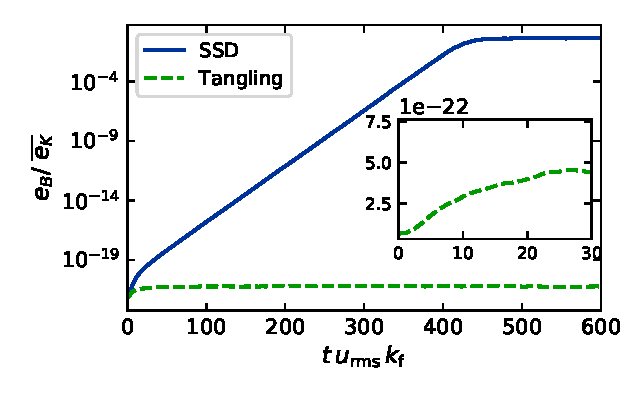
\includegraphics[trim=0.00cm 0.3cm 0.0cm 0.0cm, clip=true,width=0.91\columnwidth]{figs/ssd-tang-brms.pdf}
  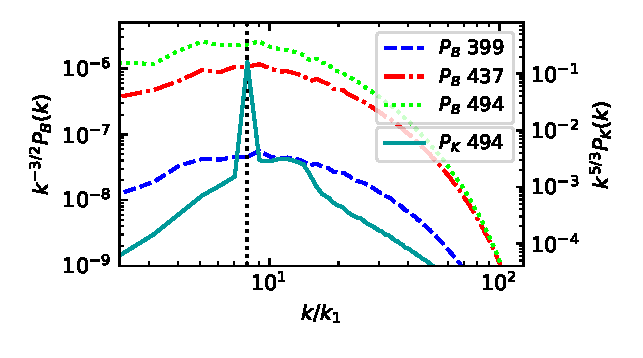
\includegraphics[trim=0.25cm 0.3cm 0.5cm 0.1cm, clip=true,width=1.0\columnwidth]{figs/ssdBpower.pdf}
  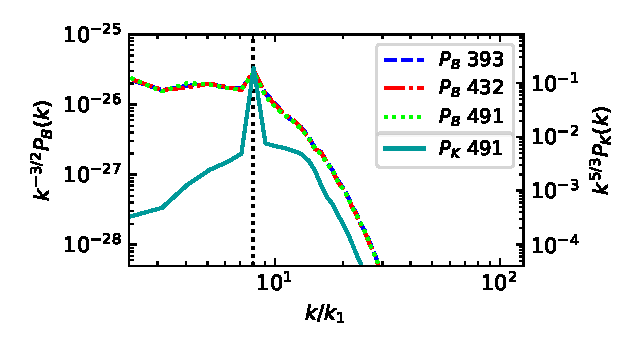
\includegraphics[trim=0.35cm 0.6cm 0.5cm 0.3cm, clip=true,width=1.0\columnwidth]{figs/tanglingBpower.pdf}
  \begin{picture}(0,0)(0,0)
    \put(0,387){{\sf\bf{(a)}}}
    \put(0,255){{\sf\bf{(b)}}}
    \put(0,125){{\sf\bf{(c)}}}
  \end{picture}
\caption{
 (a) Mean magnetic energy density, $e_B$, with nonhelical random forcing,
 scaled to time-averaged kinetic energy density, $\overline{e_K}$.
 Inset: early zoom-in of linear growth of tangled field.
 Time is normalised by eddy turnover time, $1/\kf {u_{\rm rms}}$.
 Compensated power spectra for (b) SSD and (c) tangling, at times given in the
 legends.  Note that the kinetic energy uses the right-hand axes.
  Forcing scale, $\kf/k_1=8$: vertical dotted line.
\label{fig:tangling}}
\end{figure}

%==============================================================================
\section{Disentangling the dynamo} \label{sec:ssd-tang}
%==============================================================================

 %FAG: added refs and reworded for clarity
 \fg{Previous SSD studies have examined Pm dependence with
 nonhelical forcing, including high Mach number \citep[e.g.,][]{ 
 HBD03,HBD04,Haugen:2004M,FCSBKS11,FSBS14}.}
 %To illustrate differences between tangling and SSD we adopt a simplified
 %model.
 \fg{Here, however, we adopt a simplified model purely t}o illustrate
 differences between tangling and SSD.
 Nonhelical random forcing is applied at wavenumber $\kf/k_1=8$ to
 $256^3$ zone, $2\pi$-periodic, isothermal boxes.
 The lowest wavenumber in the domain is $k_1=1$ and the largest is the Nyquist
 frequency $k/k_1 = 128$.
 The imposed uniform field has $e_B\simeq6\cdot10^{-22}~\overline{e_K}$, where
 $\overline{e_K}$ is the time-averaged kinetic energy density.
 Two simulations are distinguished by use of dimensionless
 resistivity $\eta=10^{-4}$
 and $\eta=2\cdot10^{-3}$, and viscosity $\nu=5\cdot10^{-3}$.
 These yield $\Rm=150$, with $\Pm = 50$, exciting SSD, and $\Rm=7.4$ with
 $\Pm=2.5$, inhibiting the dynamo so that amplification is limited to tangling
 of the imposed field.

 Figure\,\ref{fig:tangling}\,(a) shows the SSD growing exponentially in just over
 400 eddy turnover times; see \cite{ZRS83} for SSD properties and excitation
 conditions.
 Tangling induces only linear growth (see inset), saturating just above
 the imposed field energy within 50 turnover times.

 %FAG: edit for language
 %Power spectra for the magnetic energy of the evolving SSD and
 %tangling model are plotted
 %in Figures~\ref{fig:tangling}(b) and~\ref{fig:tangling}(c), respectively,
 %alongside a late kinetic energy spectrum.
 \fg{Power spectra of the kinetic energy and the
 evolving magnetic energy are plotted in Figures~\ref{fig:tangling}\,(b) for the
 SSD and~\ref{fig:tangling}\,(c) tangling.}
 %FAG: clearer
 %Magnetic energy spectra are compensated by Kazantsev's $k^{3/2}$
 %scaling \citep{Sch02,BS14}, and the kinetic energy by the
 %Kolmogorov's $k^{-5/3}$ spectrum.
 Magnetic energy spectra are compensated \fg{for} Kazantsev's $k^{3/2}$
 \fg{power law} \citep{Sch02,BS14}, and kinetic energy \fg{for}
 Kolmogorov's $k^{-5/3}$.
 %FAG: swapped order
 %The SSD magnetic spectrum (Figure~\ref{fig:tangling}b) experiences only a
 %slight shift of its peak to smaller wavenumber during its evolution.
 %The forcing scale $\kf$ is strongly reflected in kinetic energy and tangling 
 %magnetic energy, but does not affect the SSD magnetic spectra.
 The forcing scale $\kf$ is strongly \fg{identified} in kinetic
 energy \fg{spectra for both models} and the magnetic energy \fg{spectra of
 the tangling}, but
 \fg{is not evident in the magnetic spectra of the SSD}.
 %FAG: revised
 %The SSD magnetic spectrum (Figure~\ref{fig:tangling}b) experiences only a
 %slight shift of its peak to smaller wavenumber during its evolution.
 \fg{For SSD the range with Kazantsev power law (horizontal) extends to scales
 smaller than the forcing scale (Figure~\ref{fig:tangling}\,b), and during the
 kinematic phase the magnetic energy peak is at $k/k_1\simeq9$.}
 \fg{For tangling (Figure~\ref{fig:tangling}\,c) the Kazantsev range applies
 only at $k/k_1<\kf$.}
 %The Kazantsev range extends larger than $\kf$ for SSD, while
 %confined below $\kf$ with tangling.
 Thus, in the SSD, kinetic energy along the Kolmogorov range transfers to
 the magnetic field at these scales, inducing an inverse Kazantsev \fg{cascade}
 at scales \fg{smaller than} $\kf$, while tangling transfers energy only at
 scales between
 $\kf$ and the scale of the imposed field.
 Dissipation \fg{characterises} scales below the Kazantsev range.
 
\section{SN turbulence model design} \label{sec:model}

 %In our SN-driven turbulence models, we exclude large-scale magnetic
 %field dynamics by neglecting rotation, shear, and stratification. Our
 %simulation domain is a periodic cube of length 256 pc and zone size
 %of $\delta x=0.5$, 1, 2 or 4$\pc$.
 %A random 1~nG seed field excludes tangling of an imposed field as the 
 %source of any magnetic amplification.
 \fg{The design of these} SN-driven turbulence models, excludes large-scale
 magnetic field dynamics by \fg{omitting global scale} rotation, shear, and
 stratification.
 Our simulation domain is a periodic cube of length 256 pc and zone size
 of $\delta x=0.5$, 1, 2 or 4$\pc$\fg{, except for direct comparison with
 \BKM\  with domain 200 pc and $\delta x=0.78$, 1.56 and 3.12}.
 \fg{When comparing \BKM\ a uniform background field $\sim10$~nG is imposed.
 Otherwise we apply only a} random 1~nG seed field \fg{to} exclude tangling of
 \fg{the} imposed field as the source of any magnetic amplification.

We solve the system of non-ideal compressible MHD equations
%-------------------------------------------------------------------------------
  \begin{eqnarray}
  \label{eq:mass}
    \frac{D\rho}{Dt} &=& 
    -\rho \vect\nabla \cdot \vect{u}
    +\vect\nabla \cdot\zeta_D\vect\nabla\rho,
  \end{eqnarray}
%-------------------------------------------------------------------------------
  \begin{eqnarray}
  \label{eq:mom}
    \rho\frac{D\vect{u}}{Dt} &=& 
    \vect\nabla{\ESK\sigma}
    -\rho c_{\rm s}^2\vect\nabla\left({s}/{c_{\rm p}}+\ln\rho\right)
    +\vect{j}\times\vect{B}
    \nonumber\\
    &+&\vect\nabla\cdot \left(2\rho\nu{\mathbfss W}\right)
    +\rho\,\vect\nabla\left(\zeta_{\nu}\vect\nabla \cdot \vect{u} \right)
    \nonumber\\
    &+&\vect\nabla\cdot \left(2\rho\nu_3{\mathbfss W}^{(3)}\right)
    %FAG added correction terms
  \fg{-\vect u\vect{\nabla}\cdot\left(\zeta_D\vect{\nabla}\rho\right)},
  \end{eqnarray}
%-------------------------------------------------------------------------------
  \begin{eqnarray}
  \label{eq:ent}
    \rho T\frac{D s}{Dt} &=&
     \EST\dot\sigma +\rho\Gamma
    -\rho^2\Lambda +\eta\mu_0\vect{j}^2 
    \nonumber\\
    &+&2 \rho \nu\left|{\mathbfss W}\right|^{2}
    +\rho\,\zeta_{\nu}\left(\vect\nabla \cdot \vect{u} \right)^2
    \nonumber\\
    &+&\vect\nabla\cdot\left(\zeta_\chi\rho T\vect\nabla s\right)
    +\rho T\chi_3\vect\nabla^6 s
    %FAG added correction terms
    \nonumber\\
    &-& \fg{c_{\rm{v}}\,T \left(
    \zeta_D\nabla^2\rho + \vect\nabla\zeta_D\cdot\vect\nabla\rho\right)},
  \end{eqnarray}
%-------------------------------------------------------------------------------
  \begin{eqnarray}
  \label{eq:ind}
    \frac{\partial \vect{A}}{\partial t} &=&
    \vect{u}\times\vect{B}
    +\eta\vect\nabla^2\vect{A}
    +\eta_3\vect\nabla^6\vect{A},
  \end{eqnarray}
%-------------------------------------------------------------------------------
 with the ideal gas equation of state closing the system.
 Most variables take their usual meanings.
 %FAG added values
 Terms containing $\zeta_D\fg{=2},\,\zeta_\nu\fg{=5}$ and $\zeta\fg{_\chi=2}$
 \fg{are applied to all ISM models and} resolve shock
 discontinuities with artificial diffusion of mass, momentum, and energy
 proportional to shock strength \citep[see][for details]{GMKSH20}.
 \fg{Equations~\eqref{eq:mom} and \eqref{eq:ent} include terms with $\zeta_D$
 provide momentum and energy conserving corrections for artificial mass
 diffusion applying in \eqref{eq:mass}.}
 %Unlike \citet{Gent:2013b} shock diffusion is not applied to
 %equation~\eqref{eq:ind}, to avoid excessive magnetic dissipation in
 %shocks, which actually enhance the field by compression.
 Shock diffusion is not applied to equation~\eqref{eq:ind}\fg{, unlike
 \citet{Gent:2013b}. We avoid excessive magnetic dissipation in
 shocks, where compression actually enhances it.}
 Terms containing $\nu_3,\,\chi_3$ and $\eta_3$ apply sixth-order hyperdiffusion
 to resolve grid-scale instabilities \citep[see, e.g.,][]{ABGS02,HB04}, \fg{
 with coefficients optimal for each $\dx$}.

 %FAG para break
 %MJK Nishant's original experiments were
 %MJK solving for the continuity equation.
 %MJK Yours really not?
 %FAG: yes, I was mistaken
 %\fg{For the simplified model of the previous}
 %Sect.\,\ref{sec:ssd-tang}, we solve only equations~\eqref{eq:mom}
 %and~\eqref{eq:ind}; set $\rho=1$; do not apply shock-dependent diffusion nor
 %hyperdiffusion; and take $\vect{B}=\vect\nabla\times\vect{A}+
 %\vect{B}_{\rm imposed}$.
 \fg{The simplified isothermal model considered above
 (Sect.\,\ref{sec:ssd-tang}) solves only
 equations~\fg{\eqref{eq:mass},} \eqref{eq:mom} and~\eqref{eq:ind} but 
 without the
 shock-dependent diffusion or hyperdiffusion terms, and while setting
 $\vect{B}=\vect\nabla\times\vect{A}+\vect{B}_{\rm imposed}$.}

 \fg{In the ISM simulations} SNe are exploded at \fg{uniform} random positions
 at a Poisson rate $\dot\sigma$ \fg{proportional to} the solar neighborhood
 value $\SNr\simeq 50\kpc^{-3}\Myr^{-1}$.
 Explosions inject $\EST = 10^{51}\erg$ thermal energy, except in
 dense regions, where a proportion \fg{($<5\%$) may be} kinetic $\ESK$ 
 \citep[see][]{GMKSH20}.
 %FAG: rephrase
 %For comparability, explosions in all models with the same $\dot\sigma$ occur
 %at the same times and places.
 \fg{Models with common $\dot\sigma$ have the same timing and location of
 explosions.}
 Non-adiabatic heating $\Gamma$ and cooling $\Lambda (T)$ are included
 \citep{Gent:2013a} following \citet{Wolfire:1995} and \citet{Sarazin:1987}.

%-------------------------------------------------------------------------------
\begin{figure}
  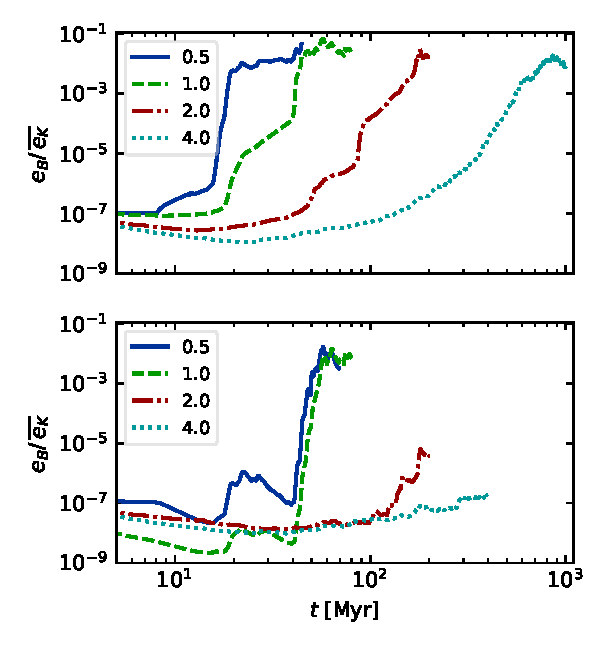
\includegraphics[trim=0.2cm 0.2cm 0.2cm 0.0cm, clip=true,width=\columnwidth]{figs/eB-res-4eta.pdf}
  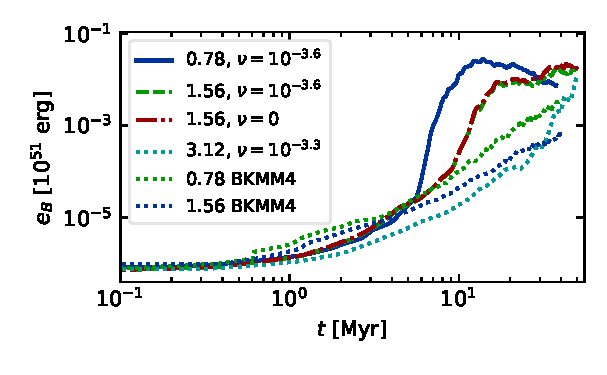
\includegraphics[trim=0.3cm 0.5cm 0.0cm 0.2cm, clip=true,width=\columnwidth]{figs/eB-Ball.pdf}
  \begin{picture}(0,0)(0,0)
    \put(210,315){{\sf\bf{(a)}}}
    \put(210,194){{\sf\bf{(b)}}}
    \put(210, 48){{\sf\bf{(c)}}}
  \end{picture}
\caption{
 Magnetic energy density,
 scaled to time-averaged kinetic energy density $\overline{e_K}$,
 for resolutions $\dx=0.5$--$4\pc$ and resistivity
 (a) $\eta=10^{-4}$ or (b) $10^{-3}$,
 \fg{and (c) matching \BKM\ scaled by $\EST$ for an imposed field with
 $\dot\sigma=8\SNr$ at $\dx=0.78$--$3.12\pc$.}
\label{fig:eb-res}}
\end{figure}
%-------------------------------------------------------------------------------

 \fg{Unlike past} experiments \citep{Gent:2013a,Gent:2013b,GMKSH20},
 thermal diffusivity, $\chi$, \fg{is omitted as} the artificial diffusivities
 are adequate to ensure numerical stability.
 \fg{The} physical effects of thermal
 conductivity can be expected to be relevant only at the unresolved or
 marginally resolved Field length defined by \citet[][named after George
 Field, not the magnetic field]{BM90}.

 %FAG: reworded without hyper to avoid confusion
 %The subset of experiments presented in this letter have viscosity $\nu=0$,
 %and hyperviscosity $\nu_3$ set optimally for each $\dx$ to ensure the flow
 %is well resolved.
 %We benchmark the magnetic field evolution by setting $\eta=0$, using only
 %hyperresistivity $\eta_3$.
 %We determine how low a physical resistivity $\eta$ can be resolved by varying
 %it from $10^{-5}$ to $10^{-3}\kpc\kms$ (units assumed henceforth).
 We \fg{isolate how numerical diffusion evolves the}
 magnetic field evolution by 
 setting $\eta=0$ \fg{and $\nu=0$.}
 We determine how low a physical resistivity $\eta$ can be resolved by varying
 it from $10^{-5}$ to $10^{-3}\kpc\kms$ (units assumed henceforth).
 \fg{We also test the effect of $\Pm=\nu/\eta$, varying $\nu$ with 
 $\eta=10^{-4}$ or varying $\eta$ with $\nu=10^{-3}$.}
 Our direct comparison with the results of \fg{\BKM} uses $\Pm=2.5$.
 
 %FAG moved to para above
 %Unlike our earlier experiments \citep{Gent:2013a,Gent:2013b,GMKSH20},
 %we do not include thermal diffusivity, $\chi$, as the artificial diffusivities
 %are adequate to ensure numerical stability and physical effects of thermal
 %conductivity can be expected to be relevant only at the unresolved or
 %marginally resolved Field length defined by \citet[][named after George
 %Field, not the magnetic field]{BM90}.

\fag{We do not address Rm in the results, although now we do include some Pm 
comparison. I have cut this section and move it after the bibliography.
 We may canabalise the relevant text for the conclusion about how Rm/Pm not
 easily related to dynamo properties in ISM}

%-------------------------------------------------------------------------------
\begin{figure*}
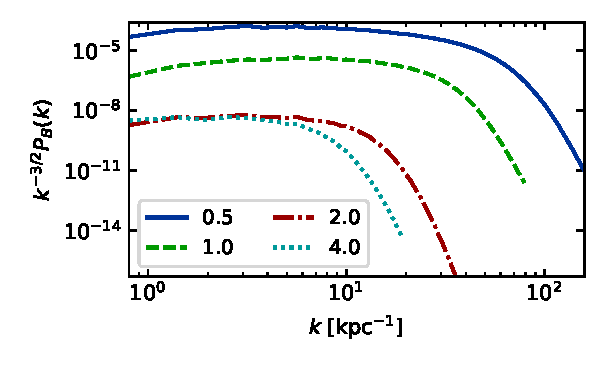
\includegraphics[trim=0 1.2cm 0 0.2cm,clip=True,width=0.48\textwidth]{figs/nu0_Bpower.pdf}
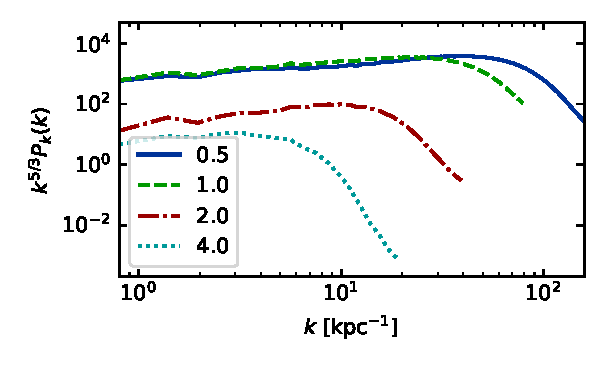
\includegraphics[trim=0 1.2cm 0 0.2cm,clip=True,width=0.48\textwidth]{figs/nu0_kpower.pdf}\\
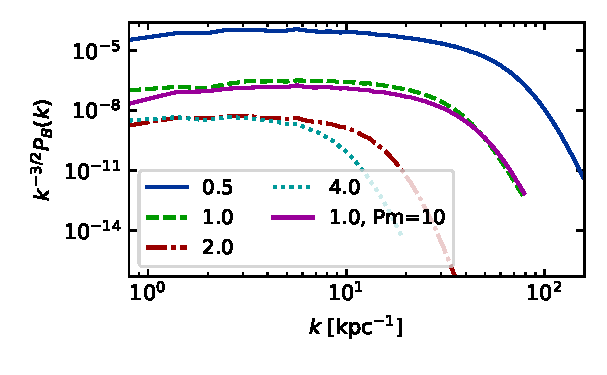
\includegraphics[trim=0 1.2cm 0 0.2cm,clip=True,width=0.48\textwidth]{figs/nu1_Bpower.pdf}
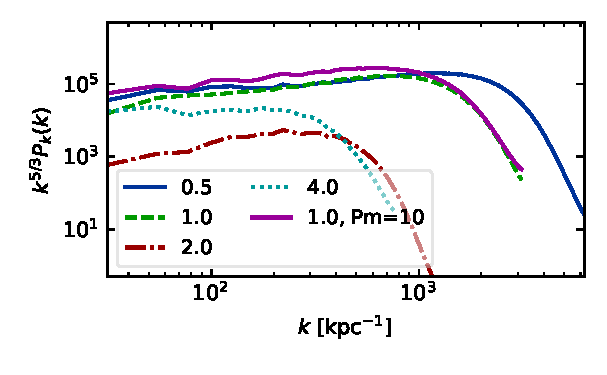
\includegraphics[trim=0 1.2cm 0 0.2cm,clip=True,width=0.48\textwidth]{figs/nu1_kpower.pdf}\\
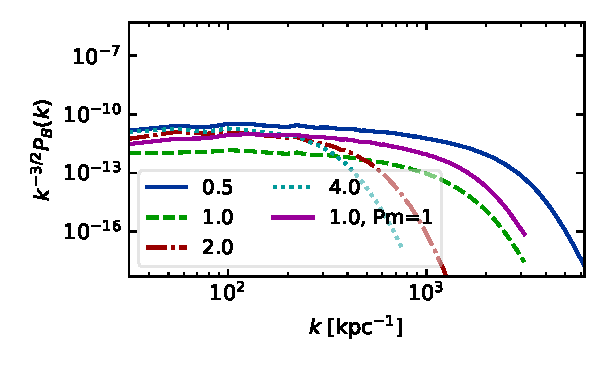
\includegraphics[trim=0 1.2cm 0 0.2cm,clip=True,width=0.48\textwidth]{figs/nu10_Bpower.pdf}
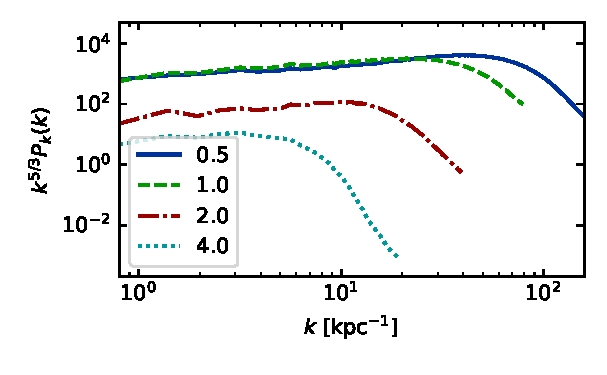
\includegraphics[trim=0 1.2cm 0 0.2cm,clip=True,width=0.48\textwidth]{figs/nu10_kpower.pdf}\\
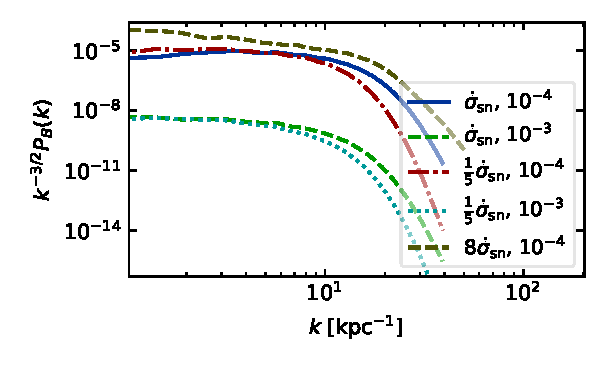
\includegraphics[trim=0 0.5cm 0 0.2cm,clip=True,width=0.48\textwidth]{figs/SN_Bpower.pdf}
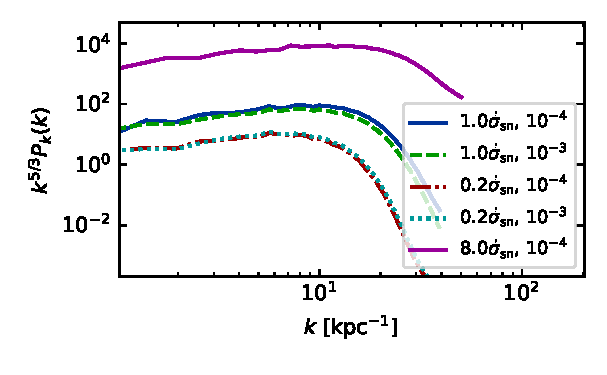
\includegraphics[trim=0 0.5cm 0 0.2cm,clip=True,width=0.48\textwidth]{figs/SN_kpower.pdf}
  \begin{picture}(0,0)(0,0)
    \put( -95,480){\begin{scriptsize}{\sf{$\eta=0$, $\dot\sigma=0.2\SNr$}}\end{scriptsize}}
    \put(-350,480){\begin{scriptsize}{\sf{$\eta=0$, $\dot\sigma=0.2\SNr$}}\end{scriptsize}}
    \put(-105,360){\begin{scriptsize}{\sf{$\eta=10^{-4}$, $\dot\sigma=0.2\SNr$}}\end{scriptsize}}
    \put(-350,360){\begin{scriptsize}{\sf{$\eta=10^{-4}$, $\dot\sigma=0.2\SNr$}}\end{scriptsize}}
    \put(-105,242){\begin{scriptsize}{\sf{$\eta=10^{-3}$, $\dot\sigma=0.2\SNr$}}\end{scriptsize}}
    \put(-350,242){\begin{scriptsize}{\sf{$\eta=10^{-3}$, $\dot\sigma=0.2\SNr$}}\end{scriptsize}}
    \put(-310,122){\begin{scriptsize}{\sf{$\dx=2\pc$}}\end{scriptsize}}
    \put( -60,122){\begin{scriptsize}{\sf{$\dx=2\pc$}}\end{scriptsize}}
    \put(-492,482){{\sf\bf{(a1)}}}
    \put(-492,358){{\sf\bf{(b1)}}}
    \put(-492,240){{\sf\bf{(c1)}}}
    \put(-492,125){{\sf\bf{(d1)}}}
    \put(-245,482){{\sf\bf{(a2)}}}
    \put(-245,358){{\sf\bf{(b2)}}}
    \put(-245,240){{\sf\bf{(c2)}}}
    \put(-245,125){{\sf\bf{(d2)}}}
  \end{picture}
\caption{
Compensated \fg{magnetic (left) and kinetic (right)} energy spectra.
Compensation is {against} the Kazantsev spectrum $k^{3/2}$ (left) or the
Kolmogorov spectrum $k^{-5/3}$ (right).
(a)--(c): \fg{Spectra are samples at $t=27.5\Myr$ for all $\dx$ for
resistivity $\eta$ and supernova rate $\dot{\sigma}$ as indicated.
$\nu=0$, except $\nu=10^{-3}$ for models identified by Pm.
(d): Samples taken for similar field strength at given $\eta$ for differing
  $\dot\sigma$ as indicated. $\dx\simeq2\pc$}  
\label{fig:3power}}
\end{figure*}
%-------------------------------------------------------------------------------


%%-------------------------------------------------------------------------------
%\section{Resolution and resistivity} \label{sec:results}
%%-------------------------------------------------------------------------------

%-------------------------------------------------------------------------------
\section{Results} \label{sec:results}
%-------------------------------------------------------------------------------

\fag{I am restructuring section 4 to deal with issues in order rather than talking about the plots in order. Hopefully this will address the referee's criticism}

%-------------------------------------------------------------------------------
\subsection{\fg{Resolution and convergence}} \label{sec:conv}
%-------------------------------------------------------------------------------

\fg{For all $\dx$ considered we find that SSD in the
 ISM appears to be easily excited.
 Figure~\ref{fig:eb-res}\,(a) for $\eta=10^{-4}$ and $\dot\sigma=0.2\SNr$
 shows growth at all $\dx$, the growth rate increasing with resolution.
 Higher numerical dissipation of the flow applies due to shock and hyper
 diffusion at low resolution, which impedes the turbulence and efficiency of
 the dynamo.
 Saturation at around 5\% of $\overline{e_K}$ appears to be a well-converged
 result.
 The growth rate does not yet quite converge between 1 and 0.5\,pc, but as we
 shall show, $\eta$ is not sufficiently acting beyond the numerical diffusion.}

 \fg{When we consider} $\eta=10^{-3}$ \fg{(Figure\,\ref{fig:eb-res}\,b), at which
 applicable resistivity is well determined by $\eta$,} there is false
 convergence
 \citep{FMA91} of solutions with similar magnetic energy decay at $\dx\geq2$.
 However, higher resolution solutions converge to rapid magnetic
 amplification occurring between 40 and 60~Myr.
 \fg{We note that strong fluctuations in the characteristics of the flow due to
 low $\dot\sigma$ and unsteady multiphase fractions induce changes in growth
 rates at higher resolution.
 There is convergence in the occurrence of sporadic slowing and acceleration
 of the dynamo for $\dx\lesssim1\pc$ and between $\eta=10^{-4}$ and $10^{-3}$,
 occurring near $t=20$ and 40\,Myr.
 }
  
 \fg{We choose low $\dot\sigma$ to preserve the multiphase structure in the 
 closed numerical domain. 
 However, we also display in Figure\,\ref{fig:eb-res}\,(c) results of direct
 comparison with \BKM\ using $\dot\sigma=8\SNr$.
 The multiphase structure rapidly fades into a single phase domain of hot gas
 ($T>10^7$\,K).
 The growth rate is faster and very uniformly exponential, reflective of the
 single phase kinematics and more persistent forcing rate, yet saturating
 also at about 5\% of $\overline{e_K}$.
 Our growth is faster than \BKM equivalent rates, because the Pencil Code is a
 higher order less diffusive code.
 We include a lower resolution run to demonstrate consistency with \BKM.
 Our runs with $\dot\sigma=\SNr$, also grow more quickly than at $0.2\SNr$,
 while saturating at $5\%\overline{e_K}$}% (Figure\,\ref{fig:eb-nu}\,f,h).}

 \fg{We can also examine the properties of the flow and magnetic field through
 their energy spectra, some of which we display in Figure\,\ref{fig:3power}.
 From panels (a2), (b2) and (c2) with kinetic spectra for all $\dx$ and 
 $\eta=0$, $10^{-4}$ and $10^{-3}$, respectively.
 Clearly there is excellent convergence in the flow for $\dx\leq1\pc$ at all
 scales $k\lesssim 30\kpc^{-1}$.
 The addition of viscosity $\nu=10^{-3}$, indicated by the magenta curves in
 panels (b2) and (c2), does not materially alter the kinetic energy spectrum
 Interestingly, the higher dissipation in the flow at the grid scale 
 $\dx\geq2\pc$ is also transferred along the whole spectrum, showing that
 the flow is losing energy even at the largest scales.
 The shape of the corresponding magnetic energy spectra are also consistent 
 for $\dx\leq1\pc$, with variation in magnitude related to differences in
 numerical resistivity.
}
 
 \fg{We have shown that SSD turbulence has convergent results for $\dx\leq1\pc$.
 Underresolving SN driven turbulence results in a significant loss of energy
 at all scales.
 SSD for $0.2\SNr\leq \dot\sigma \leq 8\SNr$ saturates in the ISM at about
 $5\%\overline{e_K}$ and grows more rapidly with increasing SN rates.
 } 


%-------------------------------------------------------------------------------
\begin{figure*}
  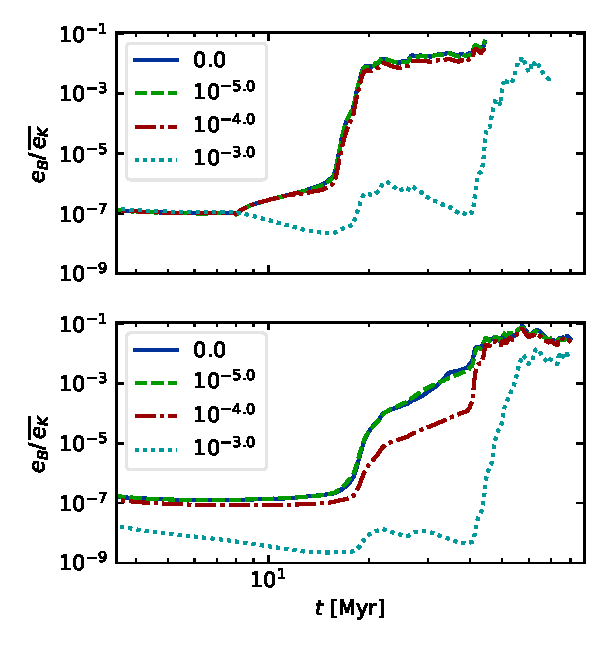
\includegraphics[trim=0.5cm 0.0cm 0.3cm 0.0cm, clip=true,width=\columnwidth]{figs/1pc-eB-nu4.pdf}
  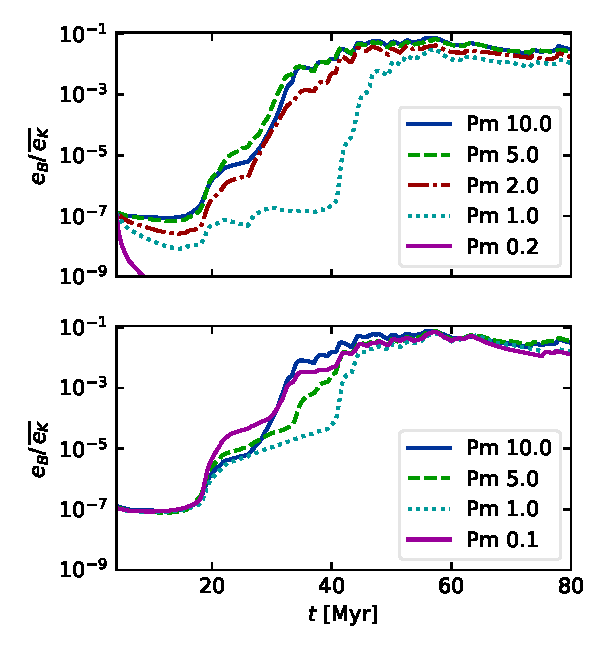
\includegraphics[trim=0.5cm 0.0cm 0.3cm 0.0cm, clip=true,width=\columnwidth]{figs/1pc-eB-nu5.pdf}\\
  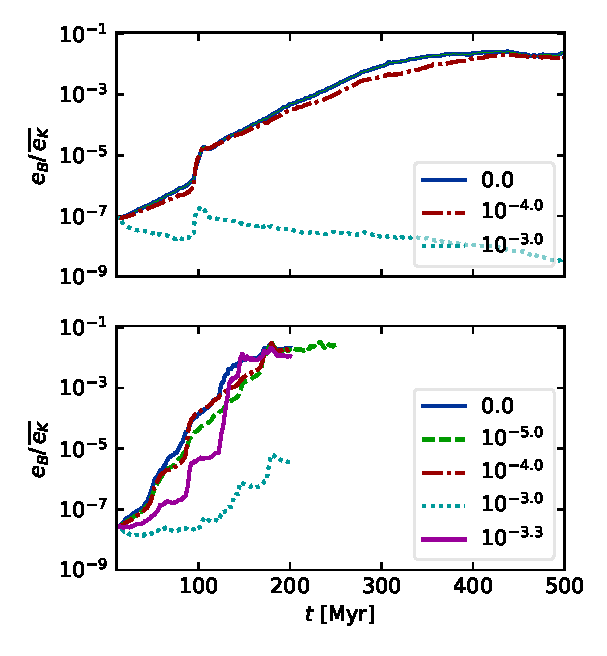
\includegraphics[trim=0.5cm 0.0cm 0.3cm 0.0cm, clip=true,width=\columnwidth]{figs/2pc-eB-nu5.pdf}
  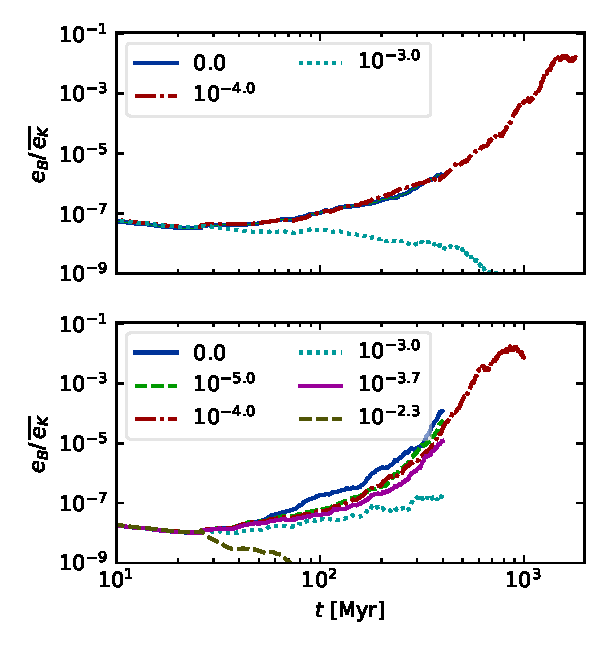
\includegraphics[trim=0.5cm 0.0cm 0.3cm 0.0cm, clip=true,width=\columnwidth]{figs/4pc-eB-nu6.pdf}
  \begin{picture}(0,0)(0,0)
    \put(-346,455){\begin{scriptsize}{\sf{$\delta x=0.5$pc, $\dot\sigma=0.2\SNr$}}\end{scriptsize}}
    \put(-100,455){\begin{scriptsize}{\sf{$\delta x=1.0$pc, $\nu=10^{-3}$}}\end{scriptsize}}
    \put(-346,330){\begin{scriptsize}{\sf{$\delta x=1.0$pc, $\dot\sigma=0.2\SNr$}}\end{scriptsize}}
    \put(-100,330){\begin{scriptsize}{\sf{$\delta x=1.0$pc, $\eta=10^{-4}$}}\end{scriptsize}}
    \put(-416,170){\begin{scriptsize}{\sf{$\delta x=2.0$pc, $\dot\sigma=0.2\SNr$}}\end{scriptsize}}
    \put(-170,170){\begin{scriptsize}{\sf{$\delta x=4.0$pc, $\dot\sigma=0.2\SNr$}}\end{scriptsize}}
    \put(-335, 45){\begin{scriptsize}{\sf{$\delta x=2.0$pc, $\dot\sigma=\SNr$}}\end{scriptsize}}
    \put( -90, 45){\begin{scriptsize}{\sf{$\delta x=4.0$pc, $\dot\sigma=\SNr$}}\end{scriptsize}}
    \put(-450,455){{\sf\bf{(a1)}}}
    \put(-450,330){{\sf\bf{(a2)}}}
    \put(-450,170){{\sf\bf{(c1)}}}
    \put(-450, 45){{\sf\bf{(c2)}}}
    \put(-205,455){{\sf\bf{(b1)}}}
    \put(-205,330){{\sf\bf{(b2)}}}
    \put(-205,170){{\sf\bf{(d1)}}}
    \put(-205, 45){{\sf\bf{(d2)}}}
  \end{picture}
\caption{
Magnetic energy density $e_B$ normalized by the time-averaged kinetic
energy $\overline{e_K}$ for various resistivities $\eta$ for values
given in each panel of resolution $\dx$ and SN rate $\dot\sigma$ normalized by
the solar neighborhood rate $\SNr\simeq 50$\,kpc$^{-3}$\,Myr$^{-1}$.
Time axes vary to accommodate SSD saturation at all $\dx$ with $\eta=10^{-4}$.
\fg{$\nu=0$, except where $\Pm=\nu/\eta$ is varied with $\nu$ fixed (c) or 
$\eta$ fixed (d).}
\label{fig:eb-nu}}
\end{figure*}
%-------------------------------------------------------------------------------
 %FAG: incorporated into new subsection on convergence of results

 %Figure~\ref{fig:eb-res}(a) shows improving convergence of dynamo growth rate
 %for $\eta=10^{-4}$ as resolution increases, although even at 0.5~pc resolution
 %full convergence does not appear to have been reached.
 %Saturation at around 5\% of $\overline{e_K}$ appears to be a well-converged
 %result.
 %At $\eta=10^{-3}$, there is false convergence \citep{FMA91} of solutions with
 %similar magnetic energy decay at $\dx=2$ and $4\pc$.
 %However, higher resolution solutions converge to rapid magnetic
 %amplification occurring between 40 and 60~Myr.
 % 
 % For $\dx\geq2\pc$ growth rates vary sporadically.
 % Growth is accelerated in Figure\,\ref{fig:eb-res}(a) and (b) near 20\,Myr,
 % 40\,Myr and again at 100\,Myr.
 % Other times show decay or lower growth rates, depending on $\dx$ or $\eta$.
 % The irregular SN forcing and varying fractional volume of different phases of
 % the ISM account for these alternating regimes, but we defer analysis of the
 % details to a future work.

%-------------------------------------------------------------------------------
\subsection{\fg{Effective resistivity and Prandtl number}} \label{sec:eta}
%-------------------------------------------------------------------------------

 \fg{To understand the role of physical parameters $\eta$ and $\nu$ on the
 SSD, we need to differentiate them from numerical diffusivities.}
 Figure~\ref{fig:eb-nu}\,(a1-a2) shows that profiles at $\eta=10^{-5}$ are
 indistinguishable from $\eta=0$, and so numerical resistivity still controls
 dynamics, even at $\delta x = 0.5\pc$.
 At $\eta=10^{-4}$ the dynamo diverges from $\eta=0$, showing that physical
 resistivity is \fg{effective}, at least in part of the domain.
 At all $\dx$ in our study physical resistivity $\eta\geq10^{-3}$ is clearly
 well resolved \fg{as the effective
 resistivity (Figure~\ref{fig:eb-nu}\,a1-d2)}.
 %FAG: true but not a significant remark
 %Models with common $\dot\sigma$ have the same schedule and location of SN,
 %but the timestep at low resolution is larger, such that actual timing and
 %explosive environment can differ between models.
 %Increased statistical noise is therefore evident, particularly in panels (e)
 %and (f).

 %FAG: this has now been commented in previous subsection. We could add details
 %FAG: from here to that paragraph, but not sure it is necessary.
 %Growth rates are sporadic within models, but are consistent between models.
 %For example, between 8 and 15\,Myr the strength of growth (or decay) in 
 %Figure\,\ref{fig:eb-nu}(a, b) reduces as $\eta$ increases.
 %Accelerated growth near 19\,Myr for $\eta=10^{-3}$ coincides with even higher
 %acceleration for $\eta\le10^{-4}$, consistent with theory.
 %The low $\eta$ models at $0.5\pc$ saturate already by 20\,Myr, but for $1\pc$
 %there is another epoch of lower growth rate up to 40\,Myr and then a
 %subsequent acceleration resulting in saturation for all models within
 %60\,Myr, including for $\eta=10^{-3}$.

 In Figure\,\ref{fig:eb-nu}(c, d) at low resolution with $\dot\sigma=0.2\SNr$
 profiles for $\eta=10^{-4}$ are not distinct from $\eta=0$, and there is no
 dynamo at all for $\dx=4\pc$ with well resolved $\eta=10^{-3}$.
 At 100\,Myr there is a period of accelerated dynamo at $\dx=2\pc$, but 
 for $\eta=10^{-3}$ this is not sustained and subsequently diffuses away.

 At $\dot\sigma=\SNr$ (Fig.\,\ref{fig:eb-nu}e, f) the higher forcing rate is
 sufficient to produce SSD at $\eta\geq10^{-3}$, but not $\eta=5\cdot10^{-3}$.
 The mean sonic Mach number $\overline\Ms=0.8$ for $\dot\sigma=\SNr$, compared
 to $0.5$ for $0.2\SNr$.
 A higher $\Ms$ has been demonstrated to impede an SSD in isothermal turbulence
 \citep{Haugen:2004M}, which is contradicted here.
 With the level of statistical noise we cannot affirm $\eta\leq10^{-4}$ exceeds
 numerical resistivity in this model. 
 However, $\eta\gtrsim5\cdot10^{-4}$ is resolved at $\dx=2\pc$ (magenta, solid)
 and at $\dx=4\pc$ the resolved limit is $2\cdot10^{-4}<\eta\lesssim10^{-3}$
 (purple, solid and cyan, dotted lines).
 For $\dx=2\pc$, (e), we see two phases of accelerated SSD at 90 and 110\,Myr,
 which are not present for $\dx=4\pc$, (f).

%-------------------------------------------------------------------------------
\begin{figure}
  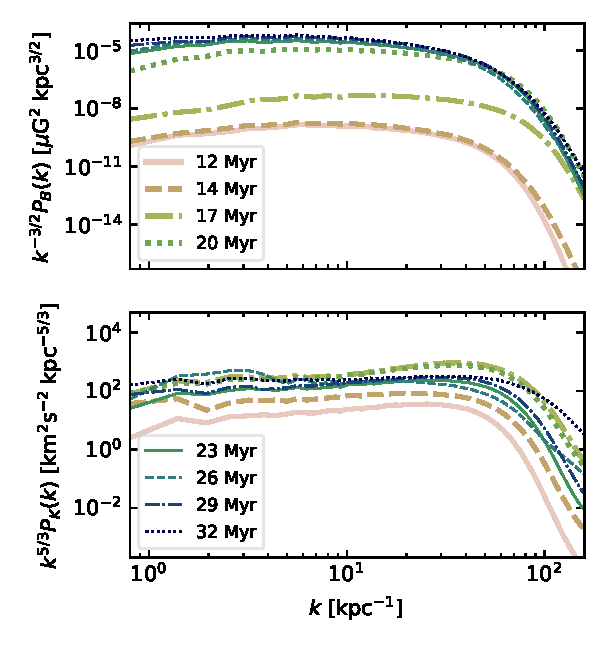
\includegraphics[trim=0.5cm 0.2cm 0.3cm 0.0cm, clip=true,width=\columnwidth]{figs/0_5pcPm0e-4_0kpower.pdf}
  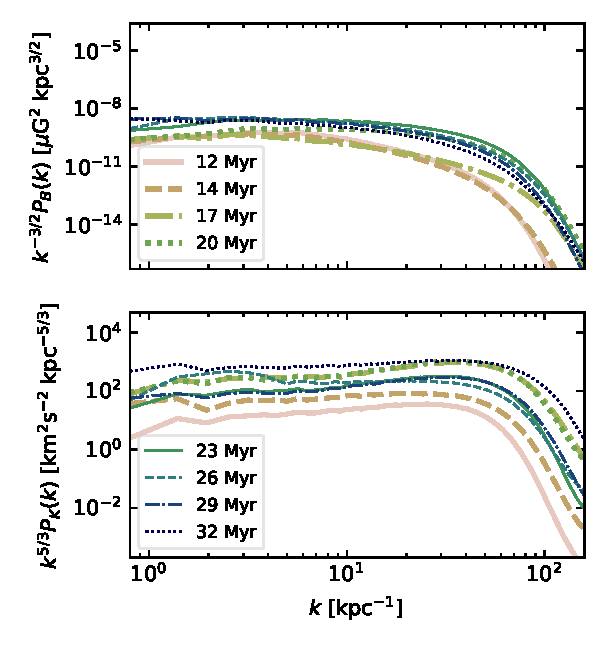
\includegraphics[trim=0.5cm 0.5cm 0.3cm 0.0cm, clip=true,width=\columnwidth]{figs/0_5pcPm0e-3_0kpower.pdf}
  \begin{picture}(0,0)(0,0)
    \put(110,455){\begin{scriptsize}{\sf{$\delta x=0.5$pc, $\nu=10^{-4}$}}\end{scriptsize}}
    \put(110,330){\begin{scriptsize}{\sf{$\delta x=0.5$pc, $\nu=10^{-4}$}}\end{scriptsize}}
    \put(110,175){\begin{scriptsize}{\sf{$\delta x=0.5$pc, $\nu=10^{-3}$}}\end{scriptsize}}
    \put(110, 50){\begin{scriptsize}{\sf{$\delta x=0.5$pc, $\nu=10^{-3}$}}\end{scriptsize}}
    \put(53,543){{\color{white}{\circle*{100}}}}
    \put(45,540){{\sf\bf{(a)}}}
    \put(45,415){{\sf\bf{(b)}}}
    \put(45,260){{\sf\bf{(c)}}}
    \put(45,135){{\sf\bf{(d)}}}
  \end{picture}
\caption{
Compensated magnetic (a, c) and kinetic (b, d) power spectra for $\dx=0.5\pc$ at times given in megayears by
the legends.  Resistivity is 
 $\eta=10^{-4}$ (a, b) or $\eta=10^{-3}$ (c, d).
Compensation is by the Kazantsev spectrum 
$k^{3/2}$ (a, c) or the Kolmogorov spectrum $k^{-5/3}$ (b, d).
\label{fig:4power}}
\end{figure}
%-------------------------------------------------------------------------------

 SN-driven turbulence does not have a well-defined forcing scale, unlike the
 simplified model in Section\,\ref{sec:ssd-tang}, because of the
 heterogeneous ISM structure and random explosions.
 The forcing scale will be distributed at scales greater than about $60\pc$
 \citep[][Table\,3]{HSSFG17}, or $k\lesssim17$~kpc$^{-1}$. 
 Figure\,\ref{fig:4power} shows the evolving compensated spectra for 
 $\dx=0.5\pc$ between 9 and 32\,Myr.
 We compare spectra for $\eta=10^{-4}$, (a, b), spanning the period of
 dynamo growth and saturation, and for $\eta=10^{-3}$, (c, d) during
 the period that the field
 persists near seed strength.
 The kinetic spectra over time match between models, until saturation
 of the dynamo at 32\,Myr (b) diminishes its energy relative to (d).
 The Kolmogorov range extends at all times to $k>20\kpc^{-1}$ and mostly 
 to $k>40\kpc^{-1}$. 

 The compensated magnetic energy spectra in Figures\,\ref{fig:4power}(a) and (c)
 have ranges conforming to the Kazantsev inverse cascade.
 For $\eta=10^{-4}$ this range extends to $k\gtrsim 20\kpc^{-1}$, above the
 forcing scale and consistent with SSD (Figure\,\ref{fig:tangling}b), until it
 contracts upon saturation to $k<10\kpc^{-1}$, consistent with no dynamo 
 (Figure\,\ref{fig:tangling}c).
 In Figure\,\ref{fig:4power}(c) the Kazantsev range occurs at $k\lesssim10$
 except for the period of 19--22\,Myr, which corresponds to a short growth
 spurt in Figure\,\ref{fig:eb-res}(b).
 The Kazantsev range does not extend to as high $k$ as the Kolmogorov range,
 a consequence of the low Pm in these SN-driven models. 
 In the high Pm ISM, where transfer from kinetic energy can occur at every
 wavenumber in the Kolmogorov spectrum, an SSD is even easier to excite.

Figure\,\ref{fig:3power}(a) -- (f) shows spectra at $t=19.5$ Myr when an SSD is
 active for the higher resolution models, and at $t=100$ Myr for the lower
 resolution models, which shows SSD for the $\dx= 2\pc$ model, but not for the
 $4\pc$ model. (Hydrodynamic parameters are fixed at each resolution.)
 The kinetic energy spectrum is convergent for $\dx=0.5\pc$ and $\dx=1\pc$,
 except for a viscous cutoff at lower $k$ for $\dx=1$.
 The kinetic energy at all $k$ is reduced for lower resolution, not just at
 the viscous dissipation scale, but even at the largest scales.
 To fully resolve the kinetic energy for scales larger than $k=24\kpc^{-1}$,
 that is $\ell\gtrsim40\pc$, therefore requires $\dx\lesssim1\pc$.
 
 The kinetic energy spectra display a bottleneck effect
 \citep{Falkovich94,HBD03}, an energy cascade less efficient than $k^{-5/3}$
 leading to an accumulation of power and then rapid dissipation at high $k$.
 This bottleneck shifts to lower $k$ as $\dx$ increases, but always at higher
 $k$ than the Kazantsev range in the corresponding magnetic spectrum, due to
 the low Pm.

 Perhaps surprisingly, there is little difference in the kinetic energy
 spectrum, Figure\,\ref{fig:3power}(h), between simulations with
 $\dot\sigma=0.2\SNr$ and $\SNr$, despite five times as much energy being
 applied to the forcing in the latter case.
 For $\eta=10^{-3}$ there is more energy near the bottleneck in the high
 $\dot\sigma$ case (cyan dotted line), so more energy can be tranferred to
 the SSD at the smallest scales.
 The comparison is obscured for $\eta=10^{-4}$, because the high $\dot\sigma$
 magnetic field is already 3 or 4 orders of magnitude stronger, acquiring some
 of the kinetic energy (red dash-dotted line).

\section{Conclusions}\label{sec:conc}

 In this Letter we demonstrate, without the use of an imposed magnetic field,
 that the field amplification demonstrated by \citet{BKMM04} was evidence of
 an SSD in SN-driven ISM turbulence and not just caused by tangling of their
 imposed field.
 Through the most extensive resolution and parameter study to date, we show
 that SN-driven turbulence easily excites an SSD even at SN rates well below the
 Galactic value.
 Our conclusion is supported by noting that the resistivity of the ISM is far
 smaller than we can resolve numerically, so the ISM is far more susceptible to
 dynamo action than our models.
 Our models with $\dx=0.5$ and $1\pc$ with $\eta=10^{-3}\kpc\kms$ show that a
 seed field of less than 1~nG can be amplified to saturation at microgauss
 levels within about 10\,Myr (Figure\,\ref{fig:eb-res}). 
 Unlike isothermal turbulence high Mach numbers do not necessarily impede SSD
 in the ISM with increasing SN forcing.

 We further show that simulations with insufficient resolution can appear to
 converge to a false solution lacking dynamo activity
 (Figure\,\ref{fig:eb-res}b). This can occur because these simulations are not
 scale independent. 
 The SN energy input and the physically motivated ISM cooling processes impose
 length and time scales that must be adequately resolved.
 To reach true convergence requires resolution of $1\pc$ or better.
 In our models, resolutions $\dx\geq2\pc$ not only give an incorrect dynamo
 solution, but also exhibit significant kinetic energy losses due to excess
 dissipation.
 This also affects the energy spectrum at the largest scales, so should be 
 considered when interpreting results using adaptive mesh refinement.
 We do, however find the well-converged result at all resolutions that when an
 SSD is excited it saturates at about 5\% of the energy equipartition level.
 At low resolution this is a lower bound, because the time-averaged kinetic
 energy density is understated, due to dissipative losses.
 This might account for the discrepancy between the energy density of the mean
 magnetic field and the random magnetic field in \citet{Gent:2013b}, due to the
 LSD being well resolved while the SSD remained underresolved.

 We find that the conventional approach from dynamo theory of categorising the 
 turbulence according to Rm based on a forcing scale $\ell$, mean random velocity
 $u_{\rm rms}$ and resistivity $\eta$ is inadequate for such a complicated
 system.
 We will show in upcoming work that the ISM appears to have multiple regimes
 with thermal phases occupying changing fractional volumes
 \citep[e.g.][]{gatto2015} and hosting SSD instabilities with different
 thresholds and growth rates.
 Explaining the interaction of these SSDs will require more sophisticated
 statistical and perhaps toplogical techniques, in advance of being able to 
 address how such an SSD interacts with an LSD.

 With grid resolution $\dx\geq2\pc$, an SSD in SN-driven turbulence simulations
 can be excluded with $\eta\gtrsim10^{-3}\kpc\kms$.
 In \citet{Gressel:2008} and \citet{GE20}, $\dx$ is 8.3 and $6.7\pc$,
 respectively and $\eta\simeq6.5\cdot10^{-3}\kpc\kms$, which appears to exclude
 an SSD.
 \citet{Gent:2013b} applied $\eta\simeq8\cdot10^{-4}\kpc\kms$ with $\dx=4\pc$,
 which would support SSD with SN rates similar to the solar neighbourhood.
 The latter obtain an LSD with galactic angular momentum $\Omega=\OSN$, where
 $\OSN=25\kms\kpc^{-1}$ is the rate in the solar neighbourhood.
 The former require $\Omega\geq4\OSN$ to excite an LSD.
 The value of Rm at the largest scales would be 7.5 times higher for the latter
 model, which alone can explain the LSD at lower $\Omega$.
 Early efforts by \citet{Korpi:1999b} were unable to detect even LSD.
 With a resolution even less than \citet{Gressel:2008} $\Omega\gg\OSN$ would
 be required to excite LSD, and SSD would be ruled out.

\acknowledgments
The authors wish to acknowledge CSC – IT Center for Science, Finland, for
computational resources Grand Challenge GDYNS Project 2001062.
M-MML was partly supported by US NSF grant AST18-15461.
FAG and MJK acknowledge support of the Academy of Finland
ReSoLVE Centre of Excellence (grant number 307411).
This project has received funding from the European Research Council (ERC)
under the European Union's Horizon 2020 research and innovation
programme (Project UniSDyn, grant agreement no: 818665).
\software{Pencil Code \citep{brandenburg2002,Pencil-JOSS}}

\bibliography{refs}{}
\bibliographystyle{aasjournal}

 A commonly used expression for Rm is 
 \begin{equation}\label{eq:sRm}
 \Rm=\frac{\ell {u_{\rm rms}}}{\eta},
 \end{equation}
 where $\ell = 2 \pi/\kf$ is the forcing scale.
 However, the inhomogeneity of the turbulence and changing multiphase
 composition of the ISM render defining a single forcing scale or rms velocity
 unreliable.
 We, therefore, consider computing Rm at each grid point directly from the
 ratio of advective to diffusive terms in the induction equation
 %-------------------------------------------------------------------------------
 \begin{eqnarray}\label{eq:Rm}
   \Rm = \frac{\left|\vect{u}\times\vect{B}\right|}{
     \left|\eta\vect\nabla^2\vect{A}+\eta_3\vect\nabla^6\vect{A}\right|}.
 \end{eqnarray}
 %-------------------------------------------------------------------------------
%FAG saved from end of section 3 
Using averaged values (eq.~[\ref{eq:sRm}]), 
 $\Rm = 1.5 \cdot 10^4$, for $\eta=10^{-4}$, $\ell=50\pc$ and
 ${u_{\rm rms}}=30\kms$.
 With the local definition (eq.~[\ref{eq:Rm}]) in the model with 
 $\dx=0.5\pc$ and $\eta=10^{-4}$ at 20\,Myr we find
 $\Rm\in(1.0\cdot10^{-4},5.8\cdot 10^3)$,
 and mean value $\langle\Rm\rangle=4.1\pm5.7$.
 Thus, the mean Rm appears unhelpful:
 in the ISM some phases and regions may exceed the critical Rm for an
 SSD while others do not.
 Microscopic resistivity is temperature dependent \citep{CSR50}.
 Even considering only turbulent resistivity to have relevance, 
 typical length scales and rms velocities differ between phases.
 Therefore, we use the explicitly chosen resistivity $\eta$ to discriminate
 between models rather than Rm.

 We have set $\nu=0$ and $\nu_3=\eta_3$ sufficient to numerically resolve the
 grid scale.
 The magnetic Prandtl number $\Pm = \Rm/\Rey$, and like $\Rm$ we have
 $\Pm\in(4.2\cdot10^{-6},4.8\cdot10^{4})$, due to inclusion of shock capturing
 viscosity and differences in definition of hyperviscosity and hyperresistivity.
 Hence, some part of each simulation will be characterised by high Pm,
 but $\langle\Pm\rangle<1$.
 This is a regime less conducive to exciting the SSD than the high $\Pm$ regime
 typical of the ISM \citep{HBD04}.
 In separate experiments with $\nu>\eta$ (high Pm), which we shall describe in
 future work, we do in fact see increased growth rates for lower $\eta$, as
 expected \citep{Sch07}.
\end{document}

